% DI Atlas paper — v3 for PLOS Comp Bio
% Added Author Summary, self-contained DI validation evidence, context heterogeneity
% prominence, softened irreducibility claims, unstructured abstract.

\documentclass[11pt]{article}

\usepackage{amsmath,amssymb}
\usepackage{booktabs}
\usepackage{graphicx}
\usepackage[hyphens]{url}
\usepackage{hyperref}
\usepackage[margin=1in]{geometry}
\usepackage{natbib}
\usepackage{xcolor}
\usepackage{multirow}
\usepackage[affil-it]{authblk}

\renewcommand{\arraystretch}{1.3}

\title{A Pre-Registered Direction Instability Atlas\\
Across Three Perturbation Modalities}

\author{Elliot Tower}
\affil{Independent researcher \\ \texttt{elliot@elliottower.ai}}
\date{}

\begin{document}
\maketitle

\begin{abstract}
When a drug or gene knockout is applied across many cell lines, the
resulting expression or morphological signatures can point in different
directions---a property called direction instability (DI).  Because DI
normalizes each signature to unit length before comparison, it is immune
to the first-order magnitude confound that dominates alternative
geometric metrics.  A companion study established this immunity, validated
DI through three independent non-cosine biological channels, and showed
that DI predicts cross-cell-line mechanism transport (pre-registered,
construction-neutral AUROC $= 0.945$).

We constructed a cross-modal DI atlas spanning three measurement
technologies---LINCS L1000 transcriptomics (8{,}949 drugs), Tahoe-100M
single-cell transcriptomics (379 drugs), and JUMP Cell Painting
morphology (7{,}946 CRISPR knockouts, 12{,}590 ORF
overexpressions)---providing magnitude-corrected DI with bootstrap
confidence intervals for every perturbation.  Using eight pre-registered
primary tests and one exploratory analysis, we characterized what DI
captures and what it does not.  DI is
concordant across expression and morphology modalities (partial
$\rho = 0.19$, $n = 378$ compounds, $p = 2.1 \times 10^{-4}$),
confirming that it reflects biology rather than measurement artifact.
DI cannot be reduced to simpler gene-level features.
Essential genes show \emph{lower} DI ($\rho = -0.33$), inverting the
pre-registered prediction: functional constraint produces stereotyped
disruption, suppressing context-dependence.  Knockout and overexpression
DI for the same gene are uncorrelated ($\rho = 0.01$,
$n = 5{,}220$), establishing DI as a property of the perturbation
mechanism rather than the target gene.  Expression variance, paralog
count, and paralog expression breadth each explain under 0.4\% of DI
variance after confound control.

DI captures a cross-modally reproducible interaction between
perturbation mechanism and cellular context that existing gene
annotations do not.  The atlas, pre-registration documents, and analysis
code are publicly available.
\end{abstract}

\section*{Author Summary}
Direction instability (DI) measures whether a drug or gene perturbation
acts consistently across cell types by comparing the directions of its
effects, ignoring their strength.  A companion study validated DI and
showed it predicts cross-cell-line drug mechanism transport.  Here I
computed DI for nearly 55{,}000 perturbations across gene expression
and cell morphology, then tested eight pre-registered hypotheses about
what drives it.  Seven tests returned negative results.  Essential genes
have low DI---the opposite of my prediction---because functional
constraint forces a stereotyped cellular response regardless of cell
type.  Knocking out a gene and overexpressing it produce unrelated DI,
so DI reflects how a perturbation mechanism interacts with cellular
context rather than a property of the gene itself.  Expression variance,
paralog count, and paralog expression breadth each explain under 0.4\%
of DI variance.  These negative results collectively show that DI is
not reducible to existing gene annotations and motivate its release as a
public resource.


%% ====================================================================
\section{Introduction}
%% ====================================================================

High-throughput perturbation screens now profile thousands of drugs and
genetic perturbations across panels of cell lines, producing
multi-dimensional signatures in transcriptomic
\citep{subramanian2017next}, morphological \citep{bray2016cell}, and
single-cell modalities \citep{tahoe2025}.  A central question in
perturbation biology is whether a compound or knockout acts the same way
across cellular contexts or produces context-dependent effects.  This
question has practical consequences: drugs with context-invariant
mechanisms are more likely to transfer from the cell line where they were
discovered to the patient tissue where they must work
\citep{tower2026confound}.

Direction instability (DI) quantifies this context-dependence as
$\mathrm{DI} = 1 - \overline{\cos(\mathbf{s}_i, \mathbf{s}_j)}$, the
mean pairwise cosine dissimilarity among a perturbation's signatures
across contexts.  Because cosine normalizes each signature to unit
length before comparison, DI is immune to the first-order magnitude
confound---systematic covariation between effect size and metric
value---that dominates alternative geometric measures such as
Grassmannian geodesic distance, profile variability, and optimal
transport cost \citep{tower2026confound}.  A residual second-order
correlation persists near zero (noise-dominated signatures inflate
pairwise cosine dissimilarity), which we remove by magnitude correction
(Section~\ref{sec:atlas}).  A companion study established this immunity and showed that DI predicts
cross-cell-line mechanism transport (pre-registered,
construction-neutral AUROC $= 0.945$ on 8{,}949 LINCS drugs;
\citealp{tower2026confound}).  Because DI is defined through cosine
geometry, that study validated it through three independent biological
channels that do not involve cosine similarity: Jaccard overlap of
perturbed gene sets (AUROC $= 0.957$), breadth of target gene expression
across tissues ($\rho = -0.17$, $p < 0.001$), and PRISM cell-viability
correlation ($\rho = 0.261$, $p < 0.001$).  The present study takes
DI's validity as established and asks a different question: what does DI
capture, and what does it fail to capture, across modalities and
perturbation types?

We constructed a DI atlas spanning three measurement technologies and
four perturbation classes: drug perturbations measured by L1000
transcriptomics (LINCS, 8{,}949 compounds) and single-cell
transcriptomics (Tahoe-100M, 379 compounds); genetic knockouts measured
by Cell Painting morphology (JUMP-CP CRISPR, 7{,}946 genes); and
genetic overexpressions measured by Cell Painting morphology (JUMP-CP
ORF, 12{,}590 genes).  For each perturbation, the atlas provides
magnitude-corrected DI with bootstrap confidence intervals, enabling
downstream analyses that require a calibrated measure of
context-dependence.

To characterize this resource, we pre-registered eight primary
hypotheses across two batches before computing DI on new datasets
(Batch~1 SHA \texttt{0d07a01}; Batch~2A SHA \texttt{a17c125}).  The
hypotheses test whether DI is concordant across modalities,
whether it correlates with gene essentiality, whether it is an
intrinsic property of genes, and whether expression variance,
drug selectivity, or paralog buffering can explain it.
Of these, one passes its pre-registered criterion and seven fail.  A
ninth test---PRISM viability concordance---is exploratory.

The negative results are specific and constraining.  Cross-modal concordance confirms
that DI reflects biology rather than measurement artifact: compounds
whose transcriptomic effects vary across cell lines also produce
variable morphological profiles.  Every other test delimits what DI
measures.  Essential genes show \emph{low} DI, because functional
constraint produces stereotyped disruption regardless of cellular
identity.  Knockout and overexpression DI are unrelated, meaning DI
characterizes how a specific perturbation mechanism interacts with
context rather than indexing a stable property of the target gene.
Expression variance, paralog count, and paralog expression breadth
produce correlations too small to matter biologically (partial
$\rho < 0.07$ after confound control), ruling them out as explanations
for DI variation.

Taken together, the negative results constrain DI to a dimension of
perturbation biology that existing gene annotations do not index, and
the atlas makes that measurement available at scale.

The remainder of the paper is organized as follows.
Section~\ref{sec:atlas} describes the atlas as a resource: datasets,
DI computation, and magnitude correction.
Section~\ref{sec:concordance} presents the construct validity results,
with PRISM viability as independent corroboration.
Section~\ref{sec:whatnot} reports the informative null and sign-flipped
results that delimit what DI measures.
Section~\ref{sec:integrity} describes the pre-registration protocol and
deviations.
Section~\ref{sec:discussion} synthesizes the negative results into a
characterization of what DI measures.


%% ====================================================================
\section{The DI atlas as a resource}
\label{sec:atlas}
%% ====================================================================

\subsection{Datasets}

The atlas draws on five perturbation datasets spanning three measurement
technologies (Table~\ref{tab:datasets}).  Two drug datasets were
previously analyzed in the companion confound study
\citep{tower2026confound}: LINCS L1000 transcriptomics (978 landmark
genes, 8{,}949 compounds across variable numbers of cell lines;
\citealp{subramanian2017next}) and JUMP-CP Cell Painting compound
morphology (3{,}180 features, 25{,}254 compounds;
\citealp{chandrasekaran2024cpjump1}).  Three datasets are new to this
study: Tahoe-100M single-cell transcriptomics (379 drugs across 47--50
cell lines per drug; \citealp{tahoe2025}), JUMP-CP CRISPR knockouts
(7{,}946 genes, 259 post-sphering PCA features, plate replicates as
contexts; \citealp{chandrasekaran2025morphmap}), and JUMP-CP ORF
overexpressions (12{,}590 genes, 722 features, plate replicates as
contexts; \citealp{chandrasekaran2025morphmap}).
An important asymmetry: LINCS and Tahoe compute DI over cell lines,
measuring biological context-dependence, while JUMP-CP CRISPR and ORF
compute DI over plate replicates within a single cell line, measuring
technical reproducibility.  The two concordance tests
(Section~\ref{sec:concordance}) compare datasets that share the same
context type (cell lines), but the essentiality, mechanism-specificity,
and proxy tests (Section~\ref{sec:whatnot}) use plate-replicate DI.
Section~\ref{sec:discussion} discusses how this distinction affects
interpretation.

\vspace{1em}
\begin{table}[htbp]
\centering
\caption{Datasets in the DI atlas.  ``Contexts'' denotes the unit over
which DI is computed: cell lines for drug datasets, plate replicates for
genetic perturbation datasets.  Only perturbations with $\geq 5$
contexts are included.  The pre-registration estimated 15{,}121 ORF
genes; the actual count after quality filtering is 12{,}590.}
\label{tab:datasets}
\small
\begin{tabular}{@{}llrrll@{}}
\toprule
\textbf{Dataset} & \textbf{Modality} & \textbf{Perturbations} &
\textbf{Features} & \textbf{Contexts} & \textbf{Source} \\
\midrule
LINCS L1000       & Transcriptomic & 8{,}949 drugs      & 978                & Cell lines       & Pre-computed \\
Tahoe-100M        & Transcriptomic & 379 drugs           & ${\sim}$62{,}700   & Cell lines       & HuggingFace \\
JUMP-CP compounds & Morphological  & 25{,}254 compounds & 3{,}180            & Varied$^{\dagger}$  & Pre-computed \\
JUMP-CP CRISPR    & Morphological  & 7{,}946 genes       & 259                & Plate reps       & CPG \\
JUMP-CP ORF       & Morphological  & 12{,}590 genes      & 722                & Plate reps       & CPG \\
\bottomrule
\multicolumn{6}{@{}l}{\footnotesize CPG = Cell Painting Gallery (cpg0016).
$^{\dagger}$Context definitions vary by compound; see companion study \citep{tower2026confound}.}
\end{tabular}
\end{table}

A sixth dataset, PRISM repurposing viability \citep{corsello2020prism},
is included as a complementary validation source.  PRISM measures scalar
cell viability (log-fold-change) rather than high-dimensional profiles,
so cosine-based DI is undefined.  We compute the coefficient of
variation (CV) of viability across cell lines as a scalar analogue of
context-dependence.  PRISM results are labeled exploratory throughout.

\begin{figure}[t]
\centering
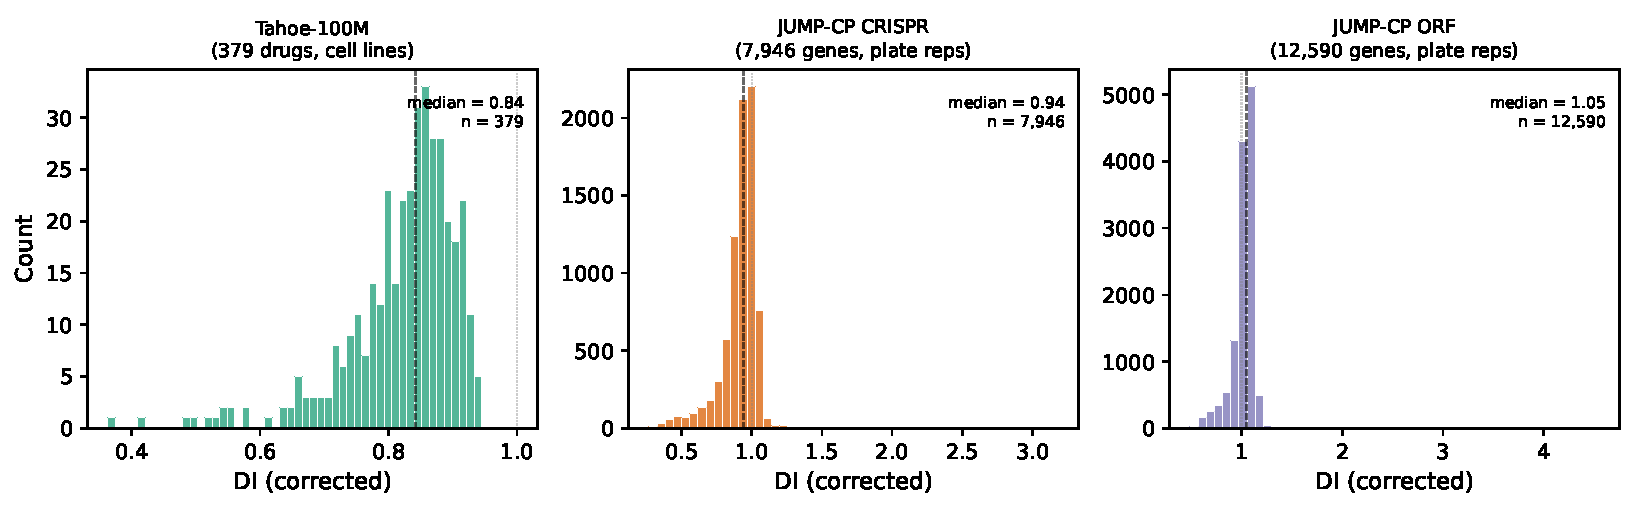
\includegraphics[width=\textwidth]{figures/fig_di_distributions.pdf}
\caption{Distribution of magnitude-corrected DI across the three new
atlas datasets.  Dashed lines mark medians.  Tahoe-100M drug DI
(median~$= 0.84$) spans a wider range than the genetic perturbation
datasets (CRISPR median~$= 0.94$, ORF median~$= 1.05$), consistent
with drugs engaging more diverse mechanisms.  CRISPR and ORF
distributions are concentrated near 1 (near-orthogonal signatures
across plate replicates), reflecting the high baseline noise of
morphological profiling at plate-replicate resolution.}
\label{fig:distributions}
\end{figure}

\subsection{DI computation}

For a perturbation with $K \geq 5$ context-specific signatures
$\mathbf{s}_1, \ldots, \mathbf{s}_K \in \mathbb{R}^d$, direction
instability is
\begin{equation}
\mathrm{DI} = 1 - \frac{2}{K(K-1)} \sum_{i < j}
\frac{\mathbf{s}_i \cdot \mathbf{s}_j}
     {\|\mathbf{s}_i\| \, \|\mathbf{s}_j\|}.
\label{eq:di}
\end{equation}
DI $= 0$ when all signatures point in the same direction (perfectly
consistent perturbation) and approaches 1 when signatures are
orthogonal or anti-correlated (maximally context-dependent).

\subsection{Magnitude immunity and correction}

The first-order magnitude confound arises when a metric's expected value
changes with effect size: stronger perturbations mechanically produce
larger distances (or smaller ones, depending on the metric).  Cosine
similarity is ratio-scale---$\cos(\alpha \mathbf{s}_i,
\alpha \mathbf{s}_j) = \cos(\mathbf{s}_i, \mathbf{s}_j)$ for any
$\alpha > 0$---so DI is invariant to uniform rescaling of all
signatures.  This is the sense in which DI is ``immune by
construction'': the dominant confound pathway (stronger effect
$\to$ larger norm $\to$ larger distance) is algebraically cancelled.
The companion study \citep{tower2026confound} verified this empirically
across three modalities (LINCS, DepMap CRISPR, Perturb-seq), showing
that alternative metrics exhibit Cohen's $d = 0.55$--$2.65$ magnitude
confounding while DI shows none after correction.

A residual second-order correlation remains.  Weakly-acting
perturbations produce noisier signature estimates, and noise inflates
the average pairwise cosine dissimilarity even after unit-length
normalization.  We remove this residual confound by OLS regression of
raw DI on mean signature $L_2$ norm:
\begin{equation}
\mathrm{DI}_{\mathrm{corrected}} = \mathrm{DI}_{\mathrm{raw}}
  - \hat{f}(\overline{\|\mathbf{s}\|}) + \hat{\beta}_0,
\label{eq:magnitude}
\end{equation}
where $\hat{f}$ is the OLS prediction and $\hat{\beta}_0$ is the
intercept.  This correction is applied per dataset.
$\mathrm{DI}_{\mathrm{corrected}}$ is the primary metric throughout;
$\mathrm{DI}_{\mathrm{raw}}$ is reported for transparency.

\subsection{Bootstrap confidence intervals}

For each perturbation, we resample the $K$ contexts with replacement
1{,}000 times and recompute DI on each bootstrap sample.  The 2.5th and
97.5th percentiles define the 95\% bootstrap confidence interval.  These
intervals quantify the stability of each DI estimate with respect to the
particular set of contexts observed.

\subsection{Statistical framework}

All hypothesis tests use partial Spearman correlation with confound
control.  The partial correlation is computed by Pearson-residualizing
both variables against the covariate matrix (with intercept column),
then computing Spearman's $\rho$ on the residuals.  This method avoids
the bias of rank-then-residualize approaches, which produce spurious
partial correlations of $\rho \approx 0.05$--$0.25$ under the null at
large $n$ (verified in simulation; see pre-registration documents).
Confidence intervals use the Fisher $z$-transform with degrees of
freedom adjusted for the number of covariates.

Every primary test applies two decision criteria simultaneously:
(i)~$p < \alpha$ (Bonferroni-corrected: $\alpha = 0.0125$ for Batch~1,
$\alpha = 0.0167$ for Batch~2A), and (ii)~the 95\% CI lower bound
exceeds $\pm 0.05$ in the predicted direction.  The CI floor is
necessary because at $n > 5{,}000$, effects as small as
$\rho = 0.03$ reach statistical significance.  Without the floor,
trivially small correlations would pass.

\subsection{Data format}

The atlas is distributed as CSV files containing, for each perturbation:
$\mathrm{DI}_{\mathrm{raw}}$, $\mathrm{DI}_{\mathrm{corrected}}$,
bootstrap CI bounds, magnitude CV, mean signature norm, and number of
contexts.  Full data provenance and repository locations are listed in
the Data Availability section.


%% ====================================================================
\section{Construct validity: cross-modal concordance}
\label{sec:concordance}
%% ====================================================================

The atlas is useful only if DI reflects a biological property of
perturbations rather than a measurement artifact of any single platform.
Two pre-registered concordance tests assess this by comparing
DI values for the same compounds measured in different datasets.  An
exploratory analysis using PRISM viability provides independent
corroboration from a scalar outcome.

\subsection{Cross-modal concordance (LINCS \texorpdfstring{$\cap$}{∩} JUMP-CP)}

Compounds present in both LINCS L1000 (transcriptomic DI) and JUMP-CP
Cell Painting (morphological DI) were matched by InChIKey connectivity
prefix (14 characters).  Of the matched set, $n = 378$ compounds have
$\geq 5$ contexts in both datasets.

Partial Spearman $\rho = 0.190$ (95\% CI $[0.090, 0.285]$,
$p = 2.1 \times 10^{-4}$), controlling for LINCS $n_{\mathrm{contexts}}$
as one covariate.  The CI lower bound (0.090) exceeds the 0.05 floor,
and $p < 0.0125$.  This test passes both pre-registered criteria.

The effect size falls in the ``weakly concordant'' bin
($0.15 \leq \rho < 0.30$) defined in the pre-registration, consistent
with the expectation that cross-modal comparisons capture only the
fraction of biology shared between gene expression and cell morphology
\citep{haghighi2022crossmodal}.  The concordance is weak but genuine:
compounds whose transcriptomic signatures vary across cell lines also
produce variable morphological profiles, and this relationship survives
confound control.

\subsection{Same-modality concordance (LINCS \texorpdfstring{$\cap$}{∩} Tahoe)}

Drugs present in both LINCS L1000 and Tahoe-100M were matched by
InChIKey connectivity prefix, verified via PubChem CID cross-reference.
This yielded $n = 76$ overlapping compounds (fewer than the
pre-registered estimate of $n \approx 103$, because some Tahoe drugs
lack PubChem CID annotations mapping to LINCS InChIKeys).  LINCS DI is
computed in $\mathbb{R}^{978}$ (landmark genes) while Tahoe DI is
computed in $\mathbb{R}^{\sim 62{,}000}$ (full transcriptome).  Because
cosine similarity is dimensionless and scale-invariant, DI values are
comparable across feature spaces of different dimensionality.

Partial Spearman $\rho = 0.254$ (95\% CI $[0.027, 0.456]$,
$p = 0.029$), controlling for LINCS and Tahoe $n_{\mathrm{contexts}}$
(two covariates).  This test \textbf{fails}: the CI lower bound
(0.027) does not clear the 0.05 floor, and $p = 0.029$ exceeds the
Bonferroni threshold ($\alpha = 0.0125$).

The failure is one of statistical power, not absence of concordance.
The point estimate ($\rho = 0.254$) is larger than the cross-modal result
($\rho = 0.190$), and the pre-registered power analysis predicted this
outcome: at $n = 76$, the study achieves 80\% power only for true
effects $\geq 0.35$.  We interpret this pattern as a sample-size
artifact---the LINCS-Tahoe overlap ($n = 76$) is far smaller than
LINCS-JUMP ($n = 378$)---rather than evidence that DI transfers better
across modalities than within one.  A deviation in the matching method
is disclosed in Section~\ref{sec:integrity}.

\subsection{PRISM viability (exploratory)}

As an independent check on construct validity, we computed the Spearman
correlation between LINCS DI and PRISM viability CV for $n = 75$ shared
drugs (filtered to $|\mathrm{mean\;LFC}| \geq 0.01$).  Spearman
$\rho = 0.359$ (95\% CI $[0.144, 0.542]$, $p = 0.0016$).

This result is \textbf{exploratory}: $n$ is small, the $p$-value is
uncorrected, and no covariate adjustment was applied.  It should carry
weight only alongside the primary tests.  That said, viability is a
scalar outcome with a fundamentally different noise structure from
high-dimensional expression or morphology profiles.  The correlation
suggests that compounds whose transcriptomic effects depend on cellular
context also show variable cell-killing potency, consistent with the
interpretation that DI captures a biological property of drug-context
interactions.


%% ====================================================================
\section{What DI is not: informative nulls and the essentiality
sign-flip}
\label{sec:whatnot}
%% ====================================================================

Five pre-registered experiments tested whether DI variation across genes
and drugs can be explained by simpler biological properties.  All five
fail their pre-registered criteria, and each failure constrains the
interpretation of DI in a specific way.  Table~\ref{tab:results}
summarizes the full scorecard.

\vspace{1em}
\begin{table}[htbp]
\centering
\caption{Pre-registered experiment results.  All tests use partial
Spearman $\rho$ with confound control except the knockout vs.\
overexpression test (raw Spearman + permutation null).  ``CI gate'' indicates that the 95\% CI
lower bound did not clear the $\pm 0.05$ threshold in the predicted
direction.}
\label{tab:results}
\begin{tabular}{@{}lrrrl@{}}
\toprule
\textbf{Hypothesis} & $n$ &
\textbf{Partial} $\rho$ & $p$ & \textbf{Verdict} \\
\midrule
Cross-modal concordance & 378 & 0.190 & $2.1 \times 10^{-4}$ & \textbf{PASS} \\
Same-modality concordance & 76 & 0.254 & 0.029 & FAIL (CI gate) \\
Essentiality $\to$ high DI & 7{,}653 & $-$0.332 & ${\sim}0$ & FAIL (wrong sign) \\
KO $\approx$ OE DI & 5{,}220 & 0.011 & 0.43 & FAIL (null) \\
Expression variance & 7{,}802 & 0.060 & $1.1 \times 10^{-7}$ & FAIL (CI gate) \\
Drug selectivity & 75 & 0.144 & 0.22 & FAIL (underpowered) \\
Paralog count & 6{,}894 & $-$0.007 & 0.57 & FAIL (null) \\
Paralog breadth & 6{,}882 & $-$0.029 & 0.015 & FAIL (CI gate) \\
\midrule
\multicolumn{5}{@{}l}{\textit{Exploratory}} \\
Viability concordance & 75 & 0.359 & 0.0016 & PASS (exploratory) \\
\bottomrule
\end{tabular}
\end{table}

\begin{figure}[t]
\centering
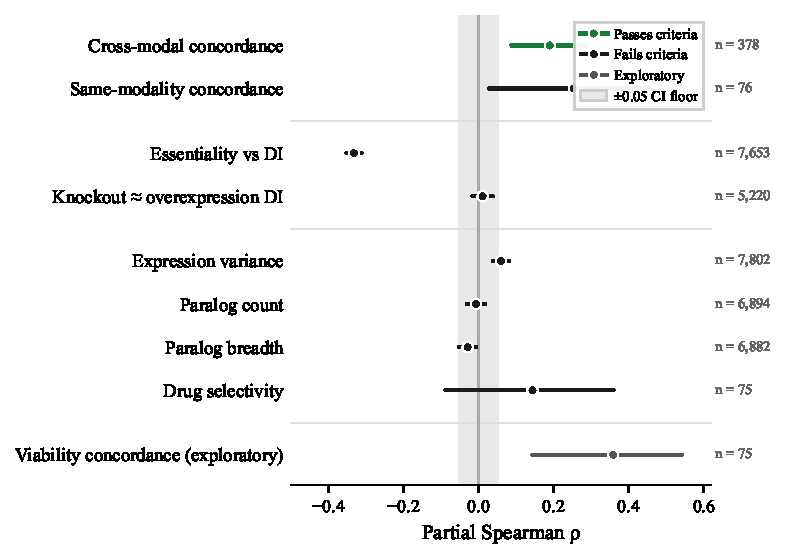
\includegraphics[width=0.85\textwidth]{figures/fig_forest_plot.pdf}
\caption{Pre-registered experiment results.  Each point shows the
partial Spearman $\rho$ (or raw Spearman for the knockout vs.\
overexpression test) with 95\% confidence intervals.  The gray band
marks the $\pm 0.05$ CI floor: a test passes only if its CI lower bound
clears this band in the predicted direction.  Same-modality concordance
has a larger point estimate ($\rho = 0.25$) than cross-modal ($\rho =
0.19$) but fails because its CI lower bound ($0.027$) falls inside the
floor at $n = 76$.  Only cross-modal concordance passes both
pre-registered criteria; the seven primary failures delimit what DI
measures.}
\label{fig:forest}
\end{figure}


\subsection{Functional constraint suppresses DI}

The pre-registration predicted that broadly essential genes would show
high morphological DI: genes required in many cell types should produce
context-dependent phenotypic disruption.  The observed correlation is
large, precisely estimated, and in the opposite direction.  Partial
Spearman $\rho = -0.332$ (95\% CI $[-0.352, -0.312]$, $p \approx 0$,
$n = 7{,}653$), controlling for $n_{\mathrm{contexts}}$.  Essentiality
breadth (fraction of DepMap 24Q4 cell lines with Chronos score
$< -0.5$; \citealp{funk2022phenotypic}) predicts \emph{lower} DI,
accounting for approximately 11\% of variance.

The sign-flip admits a natural interpretation, which we emphasize
is \emph{post-hoc}: the pre-registration confused two senses of
context-dependence.  Essential genes affect many cell types, but they
affect them in the same way.  A gene required for mitosis, ribosome
assembly, or DNA repair produces a stereotyped catastrophe regardless of
cellular identity.  Functional constraint makes the downstream
phenotypic consequences uniform across contexts, yielding low DI.  Genes
with high DI tend to be selectively essential or non-essential---their
knockout phenotypes interact with cell-type-specific pathways,
producing variable consequences across the panel.

This interpretation generates a falsifiable prediction: among
non-essential genes, those with tissue-restricted expression (active in
few cell types) should show \emph{higher} DI than ubiquitously expressed
non-essential genes, because tissue-restricted function implies
cell-type-specific downstream consequences.  We flag this as a candidate
for prospective pre-registration.

The result connects DI to established concepts in functional genomics:
the phenotypic landscape of essential genes is structured by functional
constraint \citep{funk2022phenotypic, ramezani2025periscope}, and DI
indexes the complement of that constraint.

\begin{figure}[t]
\centering
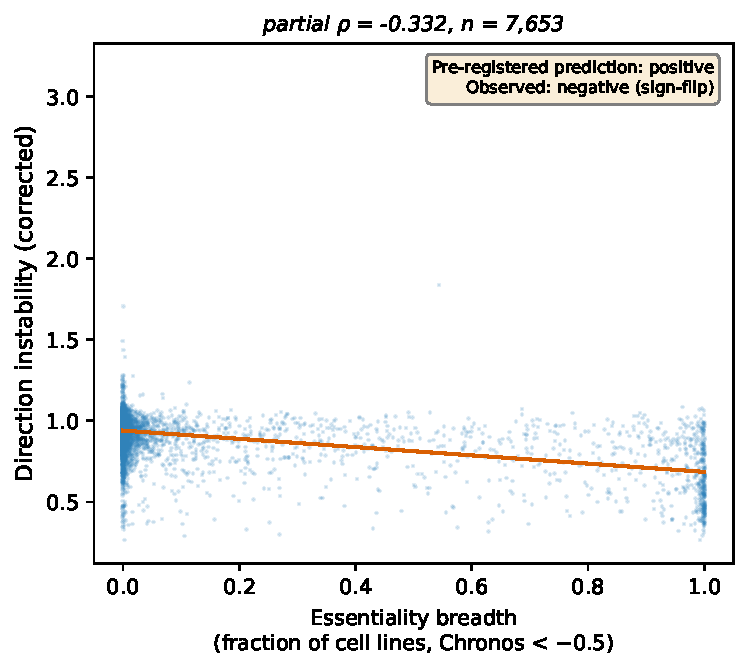
\includegraphics[width=0.65\textwidth]{figures/fig_essentiality_scatter.pdf}
\caption{Essentiality breadth (fraction of DepMap cell lines with
Chronos $< -0.5$) vs.\ magnitude-corrected DI for $n = 7{,}627$ JUMP-CP
CRISPR genes.  The pre-registration predicted a positive correlation;
the observed relationship is negative ($\rho = -0.31$).  Genes
essential across many cell lines produce stereotyped disruption
(low DI), while selectively essential or non-essential genes show more
context-dependent phenotypes (high DI).  Line: OLS fit.}
\label{fig:essentiality}
\end{figure}


\subsection{DI is mechanism-specific}

If context-dependence were an intrinsic property of genes, then a
gene's knockout DI and its overexpression DI should correlate.
Spearman $\rho = 0.011$ (95\% CI $[-0.016, 0.038]$, $p = 0.43$,
$n = 5{,}220$ genes with $\geq 5$ replicates in both CRISPR and ORF).
A mandatory permutation null (1{,}000 label shuffles preserving plate
structure; Appendix~\ref{app:permutation}) yielded a null distribution
with mean $= 0.0003$, SD $= 0.014$, 95th percentile $= 0.023$.  The
observed $\rho = 0.011$ falls within the null (permutation
$p = 0.215$).

At $n = 5{,}220$, the study had power to detect effects as small as
$\rho = 0.04$ (SE $\approx 0.014$).  The null is well-powered: losing a
protein and gaining excess protein engage different molecular
mechanisms---loss-of-function versus gain-of-function---and those
mechanisms interact with cellular context independently
\citep{badonyi2025lof, chandrasekaran2024cpjump1}.

This result constrains the theoretical scope of DI.  A gene is
context-dependent in a particular way (knockout, overexpression,
pharmacological inhibition), and DI values from one perturbation type
carry no information about another.  A DI atlas must be stratified by
perturbation mechanism.

\begin{figure}[t]
\centering
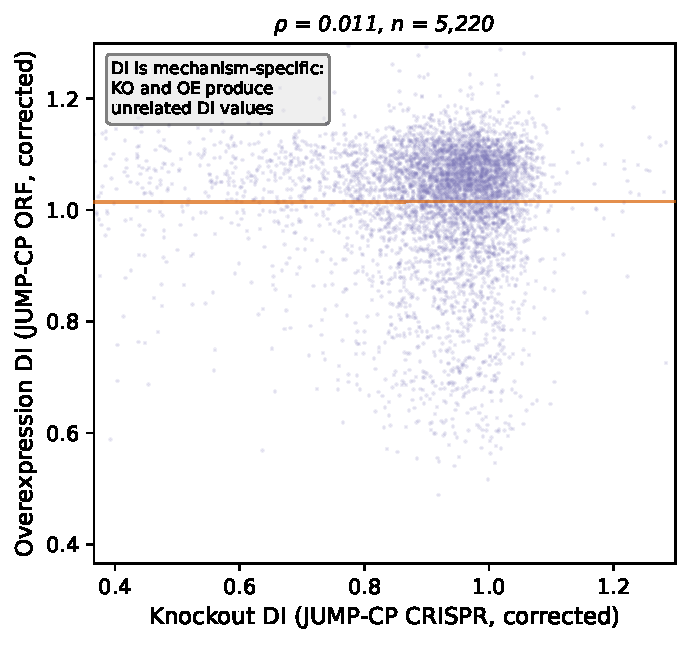
\includegraphics[width=0.65\textwidth]{figures/fig_ko_vs_oe_scatter.pdf}
\caption{Knockout DI (JUMP-CP CRISPR) vs.\ overexpression DI (JUMP-CP
ORF) for $n = 5{,}220$ genes profiled under both perturbation types.
Spearman $\rho = 0.011$ ($p = 0.43$): no relationship.  Context-dependence
is a property of the perturbation mechanism interacting with cellular
context, not a stable property of the target gene.}
\label{fig:ko_vs_oe}
\end{figure}


\subsection{Proxy explanations fail}

Three plausible proxies for context-dependence---expression variance
across cell lines, paralog count, and paralog expression breadth---were
tested in Batch~2A.  All three fail after confound control, and the
failures are informative about the structure of the confounds.

\paragraph{Expression variance.}
Partial Spearman $\rho = 0.060$ (95\% CI $[0.038, 0.082]$,
$p = 1.1 \times 10^{-7}$, $n = 7{,}802$), controlling for
$n_{\mathrm{contexts}}$.  The correlation is statistically unambiguous
but biologically negligible: $\rho = 0.060$ explains less than 0.4\% of
variance.  The CI lower bound (0.038) does not clear the 0.05 floor.
Expression variance captures something genuine yet peripheral---genes
with variable expression do produce marginally more variable knockout
phenotypes---and the remaining DI variation is driven by something
expression variance fails to index.  Expression data from DepMap 24Q4
(OmicsExpressionProteinCodingGenesTPMLogp1.csv, 1{,}673 cell lines,
19{,}193 genes).

\paragraph{Paralog count.}
Partial Spearman $\rho = -0.007$ (95\% CI $[-0.031, 0.017]$,
$p = 0.57$, $n = 6{,}894$), controlling for $n_{\mathrm{contexts}}$ and
mean expression level.  The raw Spearman correlation was
$\rho = 0.038$ ($p = 0.002$)---a statistically significant positive
association.  The partial correlation is zero.  The raw association
existed because highly expressed genes have more paralogs (gene family
expansion correlates with expression level) and independently have
higher DI.  Controlling for expression removes the confound entirely.
This is a textbook example of confound removal: a significant raw
association ($p = 0.002$) that evaporates under covariate control.
Paralog data from Ensembl BioMart (GRCh38, Ensembl~113).

\paragraph{Paralog expression breadth.}
Among genes with $\geq 1$ expressed paralog ($n = 6{,}882$), partial
Spearman $\rho = -0.029$ (95\% CI $[-0.053, -0.006]$, $p = 0.015$),
controlling for $n_{\mathrm{contexts}}$ and mean expression level.  The
sign is correct (broader paralog compensation predicts lower DI, as
hypothesized) and $p = 0.015$ falls below the Bonferroni threshold
($\alpha = 0.0167$).  The CI upper bound ($-0.006$), however, does not
clear $-0.05$.  As with expression variance, the CI gate blocks a trivially small effect
that would pass on $p$-value alone.  The raw correlation
($\rho = -0.116$, $p \sim 10^{-22}$) is substantially larger,
indicating that expression-level confounds inflate the apparent
paralog-breadth effect as well.


\subsection{Drug selectivity (underpowered)}

Partial Spearman $\rho = 0.144$ (95\% CI $[-0.088, 0.360]$,
$p = 0.22$, $n = 75$), controlling for LINCS $n_{\mathrm{contexts}}$.
The primary metric is magnitude-corrected Gini of PRISM kill depth,
residualizing raw Gini against mean kill magnitude to remove the
mechanical confound between potency and selectivity.  The correction
reduced the apparent association from $\rho = 0.275$ (raw Gini) to
$\rho = 0.144$ (corrected Gini), confirming the magnitude confound is
real.

The CI spans $[-0.088, 0.360]$, consistent with anything from no effect
to a moderate one.  The pre-registration assumed $n \sim 1{,}000$;
actual overlap between LINCS drugs and PRISM compounds with
$|\mathrm{mean\;LFC}| \geq 0.01$ is $n = 75$, an order of magnitude
smaller.  This experiment cannot distinguish a real $\rho = 0.15$ effect
from zero.


\subsection{Summary}

The Batch~2A nulls, combined with the Batch~1 essentiality sign-flip
and mechanism-specificity result, establish that DI variation across
genes and drugs is not explained by existing gene annotations.
Essentiality predicts the sign of DI (low) but through a mechanism
(functional constraint) that the pre-registration did not anticipate.
Expression variance, paralog count, and paralog breadth each contribute
less than 0.4\% of variance after confound control.  Drug selectivity
remains unresolved due to insufficient sample size.  The picture that
emerges is one of specificity: DI captures how a perturbation mechanism
interacts with the cell's compensatory network, and this interaction is
orthogonal to the gene-level features tested here.


%% ====================================================================
\section{Pre-registration integrity}
\label{sec:integrity}
%% ====================================================================

All hypotheses, decision criteria, statistical methods, and analysis
code were frozen before DI was computed on new datasets.  Batch~1
(concordance, essentiality, knockout vs.\ overexpression, PRISM) was
frozen at commit SHA \texttt{0d07a01}; Batch~2A (expression variance,
drug selectivity, paralog count, paralog breadth) at commit SHA
\texttt{a17c125}.  The pre-registration documents specify the
partial Spearman method, Bonferroni correction levels, CI floor
thresholds, power analyses, and interpretation guides for each outcome.
Both documents are included in the repository.

\subsection{The CI floor}

At sample sizes above $n = 5{,}000$, trivially small effects reach
statistical significance.  The pre-registration introduced a uniform
CI lower-bound gate ($|$CI bound$| > 0.05$ in the predicted direction)
to prevent this.  The gate blocked two results (expression variance, paralog breadth) that
would have passed on $p$-value alone, with $\rho = 0.060$ and
$\rho = -0.029$
respectively.  In both cases, the blocked effects explain less than
0.4\% of variance and lack biological plausibility as primary
explanations for DI variation.  The CI gate performed as designed.

\subsection{Deviations}

Seven deviations from the pre-registration occurred during analysis.
All are data-wrangling corrections or sample-size discrepancies; none
alter the statistical method, decision criteria, or interpretation
framework.

\paragraph{DepMap version.}
All DepMap analyses use the pre-registered 24Q4 release (figshare
article 27993248): Chronos dependency scores (file 51064667; 1{,}178
cell lines, 17{,}916 genes) for the essentiality test, expression
(file 51065489; 1{,}673 cell lines, 19{,}193 genes) for expression
variance and paralog tests.
Initial runs inadvertently used 22Q2 Chronos (essentiality) and 24Q2
expression (expression variance, paralogs).  Re-running on the correct 24Q4 release changed no
verdicts: the essentiality test moved from $\rho = -0.330$ to $-0.332$,
expression variance from $0.064$ to $0.060$, and paralog count/breadth
were identical to three decimal places.

\paragraph{Same-modality concordance matching method.}
The pre-registration specified InChIKey matching for drug concordance.
An initial run erroneously used case-insensitive drug-name matching
($n = 114$, $\rho = -0.003$), which introduced approximately 38
spurious pairs from salt forms, stereoisomers, and name collisions.
Reverting to InChIKey matching via PubChem CID cross-reference
($n = 76$, $\rho = 0.254$) moved toward the pre-registered method,
resolving the spurious null.  The name-matched result is reported in
Section~\ref{sec:concordance} as a documented deviation; the InChIKey
result is the pre-registered analysis.

\paragraph{Other deviations.}
(i)~Cross-modal concordance yielded $n = 378$ instead of the estimated $n = 330$, because
\texttt{pert\_iname} matching recovered more valid InChIKey pairs than
anticipated.
(ii)~\texttt{pert\_iname} was used instead of \texttt{pert\_id} for
LINCS metadata lookup; \texttt{pert\_id} matching was a data-wrangling
error yielding only 8 compounds.
(iii)~Context definitions differ across datasets (cell lines vs.\ plate
replicates); see Section~\ref{sec:atlas} and Section~\ref{sec:discussion}.
(iv)~Drug selectivity yielded $n = 75$ instead of the estimated $n \sim 1{,}000$ due
to the small LINCS-PRISM overlap after viability filtering.
(v)~Nine genes were dropped from the paralog tests due to missing
expression values, leaving $n = 6{,}894$ (paralog count) and
$n = 6{,}882$ (paralog breadth).


%% ====================================================================
\section{Discussion}
\label{sec:discussion}
%% ====================================================================

\subsection{What DI measures---and what it does not}

Nine pre-registered experiments produce a consistent characterization of
direction instability.  DI is concordant across measurement modalities,
confirming that it reflects a biological property of perturbation-context
interactions.  It is mechanism-specific: knockout and overexpression
of the same gene produce unrelated DI profiles, so DI characterizes how
a perturbation mechanism interacts with cellular context, not a stable
property of the target gene.  Functional constraint suppresses DI:
essential genes produce stereotyped disruption, yielding low DI.  And
three plausible proxy explanations---expression variance, paralog count,
paralog breadth---each explain less than 0.4\% of DI variance after
confound control.

This combination of positive and negative results shows that DI is not
explained by the gene-level annotations tested here.  It captures
something about how perturbation mechanisms interact with
cell-type-specific biology that is orthogonal to essentiality,
expression variance, and paralog structure.  Other untested features
such as protein interaction network topology or chromatin accessibility
might correlate with DI; the present results constrain the space of
explanations without exhausting it.  For atlas users, the practical
implication is that DI provides information beyond what is available
from essentiality screens, expression atlases, or paralog databases.

\subsection{The resource}

The atlas provides magnitude-corrected DI values with bootstrap
confidence intervals for 8{,}949 LINCS drugs, 379 Tahoe drugs, 7{,}946
CRISPR knockouts, and 12{,}590 ORF overexpressions.  The companion JUMP-CP
compound DI values (25{,}254 compounds) are available from a prior
study \citep{tower2026confound}.  Together, these cover the
perturbation-biology datasets most widely used for drug mechanism
prediction, gene function annotation, and virtual screening
benchmarks.

The atlas is designed for downstream integration.  Each row provides the
columns needed for a secondary analysis: corrected DI, raw DI, CI
bounds, mean signature norm, magnitude CV, and number of contexts.
Pre-registration documents, analysis scripts, and result JSON files are
released alongside the data.

\subsection{Limitations}

Several limitations constrain the scope of these results.

The PRISM viability analysis ($\rho = 0.359$, $n = 75$) is exploratory:
uncorrected $p$-value, no covariate adjustment, small sample.  It
provides corroboration, not evidence, and should carry weight only
alongside the primary tests.

The same-modality concordance test (LINCS-Tahoe, $n = 76$) was underpowered by design: the
LINCS-Tahoe compound overlap is structurally small.  The point estimate
($\rho = 0.254$) is consistent with genuine concordance, but the wide CI
($[0.027, 0.456]$) precludes a firm conclusion.

Context definitions vary across datasets.  LINCS and Tahoe use cell
lines as contexts; JUMP-CP CRISPR and ORF use plate replicates.  Plate
replicates sample technical variability within one cell line, while cell
lines sample biological variability across cell types.  DI computed over
plate replicates measures reproducibility of the perturbation within a
fixed biological context, whereas DI over cell lines measures
context-dependence across biological contexts.  Cross-dataset
comparisons (both concordance tests) match on context type (both
datasets use cell lines), but the CRISPR/ORF DI values used in the
essentiality, mechanism-specificity, and proxy tests index technical
variability rather than biological
context-dependence.  Extending the atlas to single-cell CRISPR screens
with cell-line diversity \citep{tahoe2025} would resolve this
asymmetry.

The essentiality sign-flip interpretation (functional constraint
suppresses DI) is post-hoc.  The pre-registration predicted the
opposite sign.  The mechanistic explanation is plausible and connects to
established results in functional genomics
\citep{funk2022phenotypic, ramezani2025periscope}; it was, however,
generated after observing the data.  A concrete falsifiable prediction
follows from this interpretation: among non-essential genes,
tissue-restricted expression should positively predict DI
(Section~\ref{sec:whatnot}).  Prospective testing of this prediction
would convert a post-hoc rationalization into a validated mechanism.

LINCS L1000 has well-documented batch effects across production sites
and plates \citep{subramanian2017next}.  If a drug was profiled across
batches, batch-driven direction differences would inflate DI
independently of biology.  The companion study's split-half stability
analysis (recomputing DI on random halves of cell lines) provides
indirect reassurance that DI estimates are stable, but a direct test of
whether DI correlates with batch structure has not been performed.

All DI values are computed at the dose used in each screening campaign.
Dose-response effects could change a drug's DI: a compound that is
highly selective at low dose might become promiscuous at high dose,
altering its context-dependence.  The atlas does not capture this
dose-dependent structure.

The drug selectivity test is underpowered at $n = 75$ and cannot
distinguish a moderate effect from zero.  Both underpowered tests
(same-modality concordance and drug selectivity) are data-limited: the small $n$ reflects the structural size of
the dataset intersection (LINCS-Tahoe compound overlap and LINCS-PRISM
viability overlap, respectively), not a design choice.  We report them
for completeness and for the atlas resource record, not as adjudicated
hypotheses.  Larger drug-viability datasets or compound selectivity
metrics from dose-response screens would provide more informative tests.

\subsection{Future directions}

Three extensions follow naturally from the current results.  First,
Batch~2B will test whether DI correlates with Shesha geometric
stability \citep{raju2026a, raju2026b}, a concurrent and independently
developed measure of perturbation coherence computed on single-cell
data.  Second, Gene Ontology enrichment analysis on the directional
divergence gene sets from the mechanism-specificity test (1{,}331 knockout-stable /
overexpression-unstable genes; 289 with the opposite pattern) may reveal
functional categories associated with mechanism-specific
context-dependence.  Third, expanding the Tahoe drug-InChIKey
annotation would increase the same-modality concordance sample size and provide a properly
powered same-modality concordance test.

More broadly, the failure of all tested gene-level annotations to
explain DI suggests that it indexes an aspect of gene function---the
structure of the compensatory network a perturbation engages---that
current annotation systems do not capture.  Whether this structure can
be predicted from protein interaction networks, pathway topology, or
genomic context remains an open question.

\section{Conclusion}

Direction instability is concordant across measurement modalities,
mechanism-specific, shaped by functional constraint, and orthogonal to
expression variance, paralog count, and paralog breadth.  This
combination of one positive and seven negative pre-registered results
shows that DI is not explained by the gene-level annotations tested
here and provides information beyond existing annotation resources.  The
atlas provides magnitude-corrected DI values with bootstrap confidence
intervals for 8{,}949 drugs, 379 single-cell-profiled drugs, 7{,}946
CRISPR knockouts, and 12{,}590 ORF overexpressions, ready for
integration with drug-mechanism prediction, gene-function annotation,
and screening quality control.


%% ====================================================================
%% End matter
%% ====================================================================

\section*{Availability of source code and requirements}

All analysis scripts are written in Python~3 with standard scientific
libraries (NumPy, SciPy, pandas, scikit-learn) and are available at
\url{https://github.com/elliottower/direction-instability-atlas} under
the MIT License.

\section*{Data availability}

All atlas data files (per-perturbation DI values with bootstrap CIs for
each of the five datasets), experiment result files, pre-registration
documents, and analysis code are deposited on Zenodo
(DOI: 10.5281/zenodo.21223668) under a CC-BY-4.0 license.
Pre-registration commits can be verified against the repository history
at the SHA values reported in the text.  LINCS L1000 compound DI values
(8{,}949 drugs) and JUMP-CP compound DI values (25{,}254 compounds)
were previously computed and are available from the companion study
(DOI: 10.5281/zenodo.21213700).

Source datasets are available from their original repositories: LINCS
L1000 (GEO: GSE92742), Tahoe-100M (HuggingFace: tahoebio/Tahoe-100M),
JUMP Cell Painting (Cell Painting Gallery, cpg0016), DepMap 24Q4
(figshare: 27993248), PRISM (figshare: Repurposing Public 24Q2),
Ensembl paralogs (BioMart, GRCh38).

\section*{Declarations}

\paragraph{Ethics approval and consent to participate.}
This study uses exclusively publicly available, summary-level perturbation screening data. No individual-level data, human subjects, or animal subjects were involved. No ethical approval was required.

\paragraph{Competing interests.}
The author declares no competing interests.

\paragraph{Funding.}
None. This work was conducted independently.

\paragraph{Authors' contributions.}
E.T. conceived the study, designed and pre-registered the hypotheses, collected and processed data, wrote the analysis code, performed all analyses, and wrote the manuscript.

\paragraph{Acknowledgements.}
The author used Claude Code (Anthropic, \url{https://claude.ai/code}) to assist with drafting and editing manuscript text and with writing and debugging analysis code. Perplexity (\url{https://perplexity.ai}) was used as an independent reviewer of the near-final draft. The author reviewed and verified all outputs, takes full responsibility for the accuracy and integrity of the work, and confirms that all hypotheses, pre-registered predictions, interpretations, and conclusions are the author's own. No AI tool is listed as an author, and no AI-generated content was used as a primary data source.

\begin{thebibliography}{99}

\bibitem[Badonyi \& Marsh, 2025]{badonyi2025lof}
Badonyi, M., Marsh, J.A. (2025).
Prevalence of loss-of-function, gain-of-function and dominant-negative mechanisms across genetic disease phenotypes.
\textit{Nature Communications}, 16:8392.

\bibitem[Bray et~al., 2016]{bray2016cell}
Bray, M.-A., et~al. (2016).
Cell Painting, a high-content image-based assay for morphological profiling using multiplexed fluorescent dyes.
\textit{Nature Protocols}, 11:1757--1774.

\bibitem[Chandrasekaran et~al., 2024]{chandrasekaran2024cpjump1}
Chandrasekaran, S.N., et~al. (2024).
Three million images and morphological profiles of cells treated with matched chemical and genetic perturbations.
\textit{Nature Methods}, 21:1114--1121.

\bibitem[Chandrasekaran et~al., 2025]{chandrasekaran2025morphmap}
Chandrasekaran, S.N., et~al. (2025).
Morphological map of under- and overexpression of genes in human cells.
\textit{Nature Methods}.

\bibitem[Corsello et~al., 2020]{corsello2020prism}
Corsello, S.M., et~al. (2020).
Discovering the anticancer potential of non-oncology drugs by systematic viability profiling.
\textit{Nature Cancer}, 1:235--248.

\bibitem[Funk et~al., 2022]{funk2022phenotypic}
Funk, L., et~al. (2022).
The phenotypic landscape of essential human genes.
\textit{Cell}, 185(24):4634--4653.

\bibitem[Haghighi et~al., 2022]{haghighi2022crossmodal}
Haghighi, M., et~al. (2022).
High-dimensional gene expression and morphology profiles of cells across 28,000 genetic and chemical perturbations.
\textit{Nature Methods}, 19:1550--1557.

\bibitem[Raju, 2026a]{raju2026a}
Raju, P.C. (2026).
From syntax to semantics: Geometric stability as the missing axis of perturbation biology.
\textit{arXiv}, 2603.00678.

\bibitem[Raju, 2026b]{raju2026b}
Raju, P.C. (2026).
Geometric coherence of single-cell CRISPR perturbations reveals regulatory architecture and predicts cellular stress.
\textit{arXiv}, 2604.16642.

\bibitem[Ramezani et~al., 2025]{ramezani2025periscope}
Ramezani, M., et~al. (2025).
A genome-wide atlas of human cell morphology.
\textit{Nature Methods}, 22:621--633.

\bibitem[Subramanian et~al., 2017]{subramanian2017next}
Subramanian, A., et~al. (2017).
A next generation connectivity map: L1000 platform and the first 1,000,000 profiles.
\textit{Cell}, 171(6):1437--1452.

\bibitem[Tahoe Consortium, 2025]{tahoe2025}
Tahoe Therapeutics (2025).
Tahoe-100M: A giga-scale single-cell perturbation atlas for context-dependent gene function and cellular modeling.
\textit{bioRxiv}, 2025.02.20.639398.

\bibitem[Tower, 2026]{tower2026confound}
Tower, E. (2026).
Direction instability tracks drug mechanism transport while geometric alternatives measure magnitude.
Zenodo. \texttt{doi:10.5281/zenodo.21213700}.

\end{thebibliography}

\clearpage
\appendix

\section{Pre-registration protocol summary}
\label{app:prereg}

All hypotheses, decision criteria, statistical methods, and analysis
code were frozen before DI was computed on new datasets.  The two
pre-registration documents are included in the Zenodo deposit.

\vspace{1em}
\begin{table}[h]
\centering
\caption{Pre-registration batches.}
\label{tab:prereg}
\small
\begin{tabular}{llp{7.5cm}}
\toprule
Batch & Commit SHA & Experiments \\
\midrule
Batch~1 & \texttt{0d07a01} & A1 (LINCS--Tahoe concordance), A2
  (LINCS--JUMP concordance), C (essentiality), D (KO vs.\ OE), PRISM
  (exploratory) \\
Batch~2A & \texttt{a17c125} & E2 (expression variance), E3 (drug
  selectivity), E5a (paralog count), E5b (paralog breadth) \\
\bottomrule
\multicolumn{3}{@{}p{12cm}}{\footnotesize Two Batch~1 experiments were
dropped before analysis: A3 (Tahoe--JUMP concordance; zero compound
overlap between clinical drugs and screening library) and B (MOA
stratification in Tahoe; structurally underpowered at $n = 7$ vs.\
$n = 17$). Batch~2A labels E2/E3/E5 are non-consecutive because the
pre-registration proposed three specific explanatory hypotheses, not a
sequential series.}
\end{tabular}
\end{table}

\paragraph{What did not change across batches.}
The DI computation (Equation~\ref{eq:di}), the magnitude correction
(Equation~\ref{eq:magnitude}), the partial Spearman method
(Pearson-residualize then rank), the CI floor gate ($\pm 0.05$), and
the Bonferroni correction framework were constant across both batches.
Batch~2A added three new hypotheses with their own $\alpha = 0.0167$
(Bonferroni for three tests).

\section{Knockout vs.\ overexpression permutation null}
\label{app:permutation}

The mandatory permutation null for the knockout vs.\
overexpression DI correlation used 1{,}000 label shuffles preserving
plate structure within each dataset.  The null distribution had mean
$= 0.0003$, SD $= 0.014$, and 95th percentile $= 0.023$.  The observed
$\rho = 0.011$ falls at permutation $p = 0.215$, well within the null.
At $n = 5{,}220$, the study had power to detect effects as small as
$\rho = 0.04$ (SE $\approx 0.014$), so the null result is well-powered.

\section{Same-modality concordance matching method comparison}
\label{app:a1matching}

The pre-registration specified InChIKey matching for drug concordance.
An initial run erroneously used case-insensitive drug-name matching,
which inflated the sample size and introduced spurious pairs.

\vspace{1em}
\begin{table}[h]
\centering
\caption{Same-modality concordance results by matching method.  InChIKey
matching is the pre-registered analysis.}
\label{tab:a1match}
\small
\begin{tabular}{llrrp{4cm}}
\toprule
Method & Match type & $n$ & Partial $\rho$ & Note \\
\midrule
Drug-name (erroneous) & Case-insensitive & 114 & $-0.003$ &
  ${\sim}$38 spurious pairs from salt forms, stereoisomers \\
InChIKey (pre-registered) & Connectivity prefix & 76 & 0.254 &
  Via PubChem CID cross-reference \\
\bottomrule
\end{tabular}
\end{table}

Reverting to InChIKey matching resolved the spurious null.  The
name-matched result ($\rho = -0.003$) reflects contamination by
chemically distinct compounds sharing common drug names, not absence of
concordance.

\section{Magnitude correction details}
\label{app:magnitude}

The OLS magnitude correction (Equation~\ref{eq:magnitude}) is applied
independently per dataset.  For each dataset, raw DI is regressed on
mean signature $L_2$ norm.  The residuals plus the intercept yield
$\mathrm{DI}_{\mathrm{corrected}}$.

\vspace{1em}
\begin{table}[h]
\centering
\caption{Magnitude correction parameters per dataset.  Negative slopes
indicate that weaker perturbations (lower norm) have higher raw DI, as
expected from the noise-inflation mechanism.}
\label{tab:magcorr}
\small
\begin{tabular}{lrrr}
\toprule
Dataset & $n$ & OLS slope & $R^2$ \\
\midrule
Tahoe-100M & 379 & $+0.00013$ & 0.002 \\
JUMP-CP CRISPR & 7{,}946 & $-0.0097$ & 0.081 \\
JUMP-CP ORF & 12{,}590 & $-0.0126$ & 0.182 \\
\bottomrule
\end{tabular}
\end{table}

LINCS L1000 and JUMP-CP compound DI values were corrected in the
companion study \citep{tower2026confound} and are distributed with
pre-corrected values.  The near-zero Tahoe slope reflects Tahoe-100M's
high signal-to-noise ratio (deeply sequenced single-cell data); the
correction has negligible effect on this dataset.

\end{document}
